% !TEX program = pdflatex
\documentclass[aspectratio=169,11pt]{beamer}

\usetheme{Madrid}
\usecolortheme{seahorse}
\setbeamertemplate{navigation symbols}{}
\setbeamertemplate{footline}[frame number]

\usepackage[T1]{fontenc}
\usepackage{lmodern}
\usepackage{listings}
\usepackage{booktabs}
\usepackage{tikz}
\usetikzlibrary{arrows.meta,positioning}

\lstset{
  basicstyle=\ttfamily\scriptsize,
  keywordstyle=\color{blue!70!black}\bfseries,
  commentstyle=\color{green!50!black},
  stringstyle=\color{red!60!black},
  breaklines=true,
  showstringspaces=false,
  columns=fullflexible,
  frame=single,
  backgroundcolor=\color{gray!8},
  rulecolor=\color{gray!40},
  xleftmargin=2pt,
  xrightmargin=2pt,
}

\definecolor{beastblue}{RGB}{40,80,140}
\definecolor{beastorange}{RGB}{200,100,20}
\setbeamercolor{frametitle}{fg=beastblue}
\setbeamercolor{title}{fg=beastblue}
\setbeamercolor{structure}{fg=beastblue}

\newcommand{\pkg}[1]{\texttt{\color{beastorange}#1}}
\newcommand{\code}[1]{\texttt{#1}}

\usepackage[normalem]{ulem} % for \sout

\title{BEAST 3 Overview}
\subtitle{Modernising the Build, the Type System, and the Package Ecosystem}
\author{BEAST Core Developer Team}
\date{2026}

\begin{document}

% ============================================================
% 1. TITLE
% ============================================================

\begin{frame}
\titlepage
\end{frame}

% ============================================================
% 2. OUTLINE
% ============================================================

\begin{frame}{Outline}
\tableofcontents
\end{frame}

% ============================================================
% 3. BIG PICTURE
% ============================================================

\begin{frame}{The Big Picture}
Three pillars of change in BEAST 3:
\vspace{1em}
\begin{enumerate}
\item \textbf{Maven + JPMS}: modern build system and module isolation
\item \textbf{Strongly-typed spec system}: compile-time checked inputs and domain types
\item \textbf{New package distribution}: Maven Central JARs, module-based service discovery
\end{enumerate}
\vspace{1em}
\begin{block}{Goal}
Catch more errors at compile time, simplify dependency management, and make packages first-class citizens in the Java module system.
\end{block}
\end{frame}

% ============================================================
\section{Why Maven + JPMS?}
% ============================================================

% Motivation slides: shared between beast3-overview-talk.tex and beast3-talk.tex.
% Assumes the preamble defines: \code, \pkg, beastblue, beastorange colours,
% listings, tikz with arrows.meta and positioning.

\begin{frame}{Problems We Wanted to Solve}
\begin{columns}[T]
\begin{column}{0.48\textwidth}
\textbf{Build \& dependencies}
\begin{itemize}
\item Ant \code{build.xml}: manual JAR management, no transitive dependency resolution
\item Adding a library means hand-copying JARs and editing classpaths
\item No standard way to publish or consume packages
\end{itemize}
\end{column}
\begin{column}{0.48\textwidth}
\textbf{Classloading \& isolation}
\begin{itemize}
\item Custom classloader predates Java modules by 15+ years
\item Source of ``magic'' that confuses new developers and breaks standard tooling
\item Two packages bundling different versions of the same library can conflict
\end{itemize}
\end{column}
\end{columns}
\end{frame}

\begin{frame}{Why Maven? Dependency Management}
\begin{center}
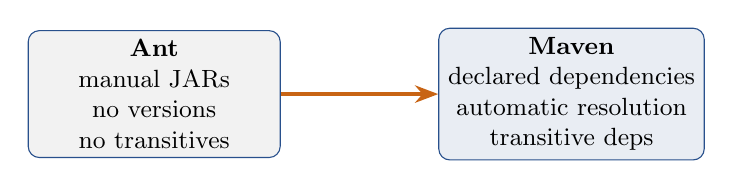
\begin{tikzpicture}[
    box/.style={draw=beastblue, rounded corners, minimum width=3.2cm, minimum height=1.2cm, align=center, font=\small},
    >=Stealth
]
\node[box, fill=gray!10] (ant) {\textbf{Ant}\\manual JARs\\no versions\\no transitives};
\node[box, fill=beastblue!10, right=2cm of ant] (mvn) {\textbf{Maven}\\declared dependencies\\automatic resolution\\transitive deps};
\draw[->, very thick, beastorange] (ant) -- (mvn);
\end{tikzpicture}
\end{center}
\vspace{0.5em}
\begin{itemize}
\item Declare what you need in \code{pom.xml}; Maven fetches, caches, and versions it
\item Transitive dependencies resolved automatically: no more ``which JARs do I need?''
\item Reproducible builds: everyone gets the same dependency tree
\end{itemize}
\end{frame}

\begin{frame}{Why Maven? Ecosystem \& Tooling}
\begin{itemize}
\item \textbf{IDE integration:} IntelliJ and Eclipse understand Maven projects natively: import, build, run, debug with zero configuration
\item \textbf{CI/CD:} GitHub Actions, Jenkins, etc.\ all have first-class Maven support
\item \textbf{Publishing:} packages can be published to Maven Central: the standard Java package registry, used by millions of projects
\item \textbf{AI-assisted development:} Copilot, agentic coding tools understand Maven projects and JPMS modules; they don't understand bespoke build systems
\item \textbf{Documentation \& community:} vast ecosystem of tutorials, StackOverflow answers, and plugins
\end{itemize}

\vspace{0.5em}
\begin{block}{}
Moving to Maven means BEAST developers benefit from the entire Java ecosystem's tooling instead of maintaining our own.
\end{block}
\end{frame}

\begin{frame}{Why JPMS Modules?}
The \textbf{Java Platform Module System} (introduced in Java 9) gives us:

\vspace{0.5em}
\begin{enumerate}
\item \textbf{Strong encapsulation}: each module declares what it exports; internal classes are truly hidden
\item \textbf{Reliable configuration}: missing dependencies are caught at startup, not at runtime via \code{ClassNotFoundException}
\item \textbf{Per-package isolation}: each BEAST package gets its own \code{ModuleLayer}; two packages can bundle different versions of the same library without conflict
\item \textbf{No split packages}: JPMS enforces that each Java package belongs to exactly one module, so good development practices are guaranteed rather than hoped for
\item \textbf{Service discovery}: \code{module-info.java} replaces classpath scanning and \code{version.xml} as the primary way to register BEASTObjects
\end{enumerate}

\vspace{0.5em}
\begin{alertblock}{}
JPMS replaces our custom classloader with a standard Java mechanism that works with, not against, the platform.
\end{alertblock}
\end{frame}

\begin{frame}{What Was Wrong with the Custom Classloader?}
\begin{itemize}
\item Using BEAST as a \textbf{library} in other projects (e.g.\ LPhyBEAST) was nearly impossible: the custom classloader conflicts with the host application's class loading
\item Debugging class-not-found errors required \textbf{BEAST-specific knowledge} that isn't transferable to other Java projects
\item New developers and contributors faced a steep \textbf{onboarding barrier}
\end{itemize}

\vspace{1em}
\textbf{BEAST 3 fix:} JPMS \code{ModuleLayer} provides per-package isolation out of the box. Standard Java, standard tooling, no magic.
\end{frame}


% ============================================================
% 9. THREE MODULES
% ============================================================

\begin{frame}{BEAST 3 Module Architecture}
Three JPMS modules, each with its own \code{module-info.java}:

\vspace{1em}
\begin{center}
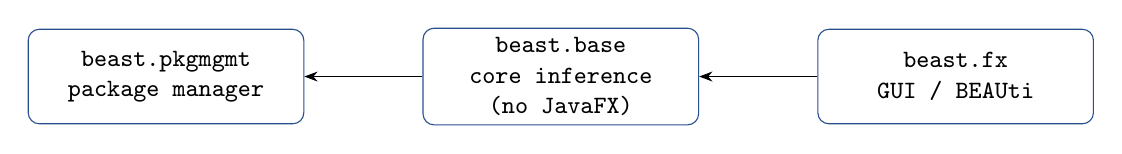
\begin{tikzpicture}[
    box/.style={draw=beastblue, rounded corners, minimum width=3.5cm, minimum height=1.2cm, align=center, font=\small\ttfamily},
    >=Stealth
]
\node[box] (pkgmgmt) {\textbf{beast.pkgmgmt}\\package manager};
\node[box, right=1.5cm of pkgmgmt] (base) {\textbf{beast.base}\\core inference\\(no JavaFX)};
\node[box, right=1.5cm of base] (fx) {\textbf{beast.fx}\\GUI / BEAUti};
\draw[->] (base) -- (pkgmgmt);
\draw[->] (fx) -- (base);
\end{tikzpicture}
\end{center}

\vspace{1em}
\begin{itemize}
\item \code{beast-base} has \textbf{no JavaFX dependency}: can run headlessly on clusters
\item JavaFX is a \textbf{Maven dependency}, not bundled with the JDK
\item All modules declared as \code{open module} (reflection OK for XML unmarshalling)
\end{itemize}
\end{frame}

% ============================================================
% 10. PROJECT STRUCTURE
% ============================================================

\begin{frame}{Project Structure}
\begin{center}
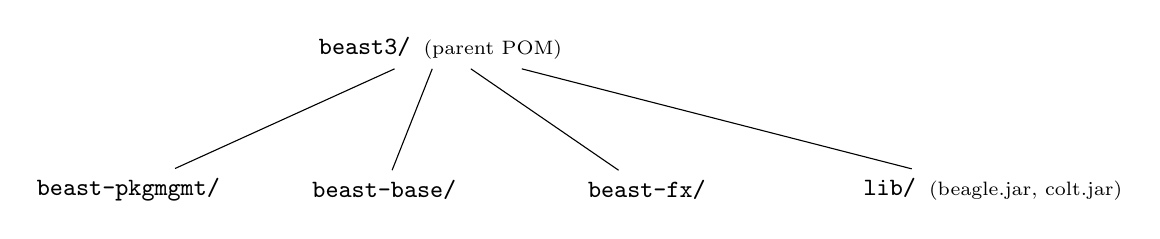
\begin{tikzpicture}[
    every node/.style={font=\small\ttfamily, anchor=west},
    level 1/.style={sibling distance=3.5cm, level distance=1.8cm},
]
\node {\textbf{beast3/} \textrm{\scriptsize(parent POM)}}
  child {node {beast-pkgmgmt/}}
  child {node {beast-base/}}
  child {node {beast-fx/}}
  child {node {lib/ \textrm{\scriptsize(beagle.jar, colt.jar)}}};
\end{tikzpicture}
\end{center}
\vspace{1em}
\begin{itemize}
\item Multi-module Maven project with a parent POM
\item \code{mvn package} builds all three modules
\item \code{beagle} and \code{colt} ship as modular JARs in \code{lib/}
\end{itemize}
\end{frame}

% ============================================================
\section{Strongly Typed Spec System}
% ============================================================

% ============================================================
% 11. TYPE SAFETY MOTIVATION
% ============================================================

\begin{frame}{The Type Safety Problem}
\textbf{In BEAST 2}, almost everything is \code{Input<RealParameter>} or \code{Input<Function>}:

\vspace{0.5em}
\begin{itemize}
\item Type errors only discovered at \textbf{runtime}: wrong parameter passed to wrong input
\item Bounds (\code{lower="0"}, \code{upper="1"}) are stringly-typed XML attributes
\item No way to express ``this must be a positive real'' in the Java API
\item IDE cannot help you: everything looks like the same type
\end{itemize}

\vspace{1em}
\begin{exampleblock}{Goal}
Make invalid models \textbf{unrepresentable} at compile time.
\end{exampleblock}
\end{frame}

% ============================================================
% 12. SPEC SYSTEM OVERVIEW
% ============================================================

\begin{frame}{Strongly Typed Parameters \& Domains}
\begin{columns}[T]
\begin{column}{0.48\textwidth}
\textbf{Typed parameters}
\begin{itemize}
\item \code{RealScalarParam}: single real
\item \code{RealVectorParam}: vector of reals
\item \code{IntScalarParam} / \code{IntVectorParam}
\item \code{BoolScalarParam} / \code{BoolVectorParam}
\item \code{SimplexParam}: probability simplex
\end{itemize}
\end{column}
\begin{column}{0.48\textwidth}
\textbf{Domain types}
\begin{itemize}
\item \code{PositiveReal}: replaces \code{lower="0"}
\item \code{UnitInterval}: replaces \code{lower="0" upper="1"}
\item \code{Real}: unbounded
\item \code{NonNegativeInt}: replaces \code{lower="0"}
\item \code{PositiveInt}: replaces \code{lower="1"}
\end{itemize}
\end{column}
\end{columns}

\vspace{1em}
\begin{itemize}
\item Domain is part of the \textbf{Java type}: compiler catches mismatches
\item Legacy classes are \textbf{deprecated, not removed}: migrate incrementally
\end{itemize}
\end{frame}

% ============================================================
% 13. BEFORE / AFTER
% ============================================================

\begin{frame}[fragile]{Before / After: Input Declaration}
\begin{columns}[T]
\begin{column}{0.48\textwidth}
\textbf{BEAST 2}
\begin{lstlisting}[language=Java]
public Input<RealParameter> kappaInput =
    new Input<>("kappa",
    "ts/tv ratio",
    Validate.REQUIRED);

// lower="0" only checked at runtime
// in the XML
\end{lstlisting}
\end{column}
\begin{column}{0.48\textwidth}
\textbf{BEAST 3}
\begin{lstlisting}[language=Java]
public Input<RealScalar<PositiveReal>>
    kappaInput = new Input<>("kappa",
    "ts/tv ratio",
    Validate.REQUIRED);

// PositiveReal is in the type!
// Compiler rejects wrong domain
\end{lstlisting}
\end{column}
\end{columns}
\end{frame}

% ============================================================
% 14. DISTRIBUTION IS THE PRIOR
% ============================================================

\begin{frame}{``Distribution IS the Prior''}
\begin{columns}[T]
\begin{column}{0.48\textwidth}
\textbf{BEAST 2}

\medskip
\code{Prior} wraps distribution + parameter:

\begin{center}
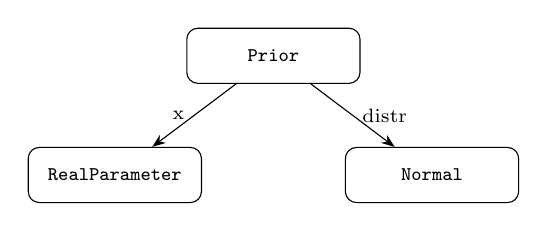
\begin{tikzpicture}[
    box/.style={draw, rounded corners, minimum width=2.2cm, minimum height=0.7cm, font=\scriptsize\ttfamily, align=center},
    >=Stealth, scale=0.9
]
\node[box] (prior) {Prior};
\node[box, below left=0.8cm and -0.2cm of prior] (param) {RealParameter};
\node[box, below right=0.8cm and -0.2cm of prior] (dist) {Normal};
\draw[->] (prior) -- node[left, font=\scriptsize]{x} (param);
\draw[->] (prior) -- node[right, font=\scriptsize]{distr} (dist);
\end{tikzpicture}
\end{center}
\end{column}
\begin{column}{0.48\textwidth}
\textbf{BEAST 3}

\medskip
Distribution \textbf{is} the prior:

\begin{center}
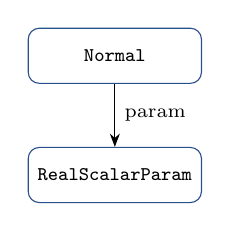
\begin{tikzpicture}[
    box/.style={draw=beastblue, rounded corners, minimum width=2.2cm, minimum height=0.7cm, font=\scriptsize\ttfamily, align=center},
    >=Stealth, scale=0.9
]
\node[box] (normal) {Normal};
\node[box, below=0.8cm of normal] (param) {RealScalarParam};
\draw[->] (normal) -- node[right, font=\scriptsize]{param} (param);
\end{tikzpicture}
\end{center}
\end{column}
\end{columns}
\vspace{1em}
Simpler model graph: no separate \code{Prior} wrapper needed.
\end{frame}

% ============================================================
\section{New Distributions \& Operators}
% ============================================================

% ============================================================
% 15. NEW DISTRIBUTIONS
% ============================================================

\begin{frame}{New Distributions \& Operators}
\begin{columns}[T]
\begin{column}{0.48\textwidth}
\textbf{New distributions}
\begin{itemize}
\item Cauchy, GammaMean
\item Bernoulli, IntUniform
\item IID (scalar $\to$ vector), 
\item OffsetReal
\item TruncatedReal
\end{itemize}
\end{column}
\begin{column}{0.48\textwidth}
\textbf{Operator changes}
\begin{itemize}
\item New \code{IntervalScaleOperator}
\item Dedicated \code{ScaleTreeOperator} (separated from \code{ScaleOperator})
\item Spec \code{UpDownOperator} replaces 3 BICEPS operators
\item Simplified default tree operator set
\end{itemize}
\end{column}
\end{columns}
\end{frame}

% ============================================================
\section{Package System}
% ============================================================

% ============================================================
% 16. PACKAGE SYSTEM OVERVIEW
% ============================================================

\begin{frame}{Package System Overview}
\begin{itemize}
\item \textbf{One ModuleLayer per package:} namespace isolation without losing visibility to the core API
\item \textbf{Same code path for dev and deployment:} \code{module-info.java} \code{provides} declarations are the single source of truth
\item \textbf{Graceful degradation:} modules with unsatisfied dependencies are silently skipped
\end{itemize}

\vspace{1em}
\begin{center}
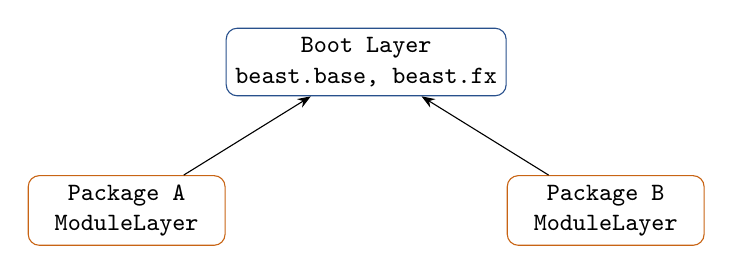
\begin{tikzpicture}[
    box/.style={draw=beastblue, rounded corners, minimum width=2.8cm, minimum height=0.8cm, font=\small\ttfamily, align=center},
    pkg/.style={draw=beastorange, rounded corners, minimum width=2.5cm, minimum height=0.8cm, font=\small\ttfamily, align=center},
    >=Stealth
]
\node[box] (boot) {Boot Layer\\beast.base, beast.fx};
\node[pkg, below left=1cm and 0cm of boot] (p1) {Package A\\ModuleLayer};
\node[pkg, below right=1cm and 0cm of boot] (p2) {Package B\\ModuleLayer};
\draw[->] (p1) -- (boot);
\draw[->] (p2) -- (boot);
\end{tikzpicture}
\end{center}
\end{frame}

% ============================================================
% 17. TWO DISTRIBUTION MODELS
% ============================================================

\begin{frame}{Package Distribution: Maven Central \& ZIP}
\begin{columns}[T]
\begin{column}{0.48\textwidth}
\textbf{Maven packages} (recommended)
\begin{itemize}
\item Published to Maven Central
\item Install via BEAUti or CLI
\item Automatic dependency resolution
\item \code{maven-packages.xml} tracks installs
\end{itemize}
\end{column}
\begin{column}{0.48\textwidth}
\textbf{ZIP packages} (legacy, still works)
\begin{itemize}
\item Traditional CBAN archives
\item One subdirectory per package
\item \code{version.xml} for service discovery
\item Self-describing directory structure
\end{itemize}
\end{column}
\end{columns}

\vspace{1em}
\begin{block}{}
Both formats coexist. Loading precedence: boot layer $\to$ Maven $\to$ ZIP.
\end{block}
\end{frame}

% ============================================================
% 18. BEAST-PACKAGE-SKELETON
% ============================================================

\begin{frame}{\code{beast-package-skeleton}}
Ready-to-copy template project on GitHub:

\vspace{0.5em}
\begin{itemize}
\item Maven \code{pom.xml} with BEAST 3 dependencies
\item \code{module-info.java} with \code{provides} declarations
\item Example distribution, operator, and tests
\item BEAST XML using the strongly-typed spec API
\item Maven Central release profile
\end{itemize}

\vspace{1em}
\begin{exampleblock}{}
\centering
Start here: \url{https://github.com/CompEvol/beast-package-skeleton}
\end{exampleblock}
\end{frame}

% ============================================================
\section{Migration \& Summary}
% ============================================================

% ============================================================
% 19. KEY CHANGES & MIGRATION
% ============================================================

\begin{frame}{Key Breaking Changes}
\begin{center}
\begin{tabular}{lll}
\toprule
\textbf{Area} & \textbf{BEAST 2} & \textbf{BEAST 3} \\
\midrule
Build & Ant, Java 8/11 & Maven, Java 25 \\
Modules & Custom classloader & JPMS \code{ModuleLayer} \\
Parameters & \code{RealParameter} & Typed spec params + domains \\
Priors & \code{Prior} wrapper & Distribution is the prior \\
\code{StateNode} & implements \code{Function} & No longer a \code{Function} \\
\code{StateNode.scale()} & built-in & Removed; use \code{Scalable} \\
JavaFX & Bundled with JDK & Maven dependency \\
\bottomrule
\end{tabular}
\end{center}

\vspace{0.5em}
Legacy classes are \textbf{deprecated, not removed}: migrate incrementally.
\end{frame}

% Timeline slide: shared between beast3-overview-talk.tex and beast3-talk.tex.
% Assumes the preamble defines: beastblue, beastorange colours,
% tikz with arrows.meta and positioning.

\begin{frame}{Timeline}
\begin{center}
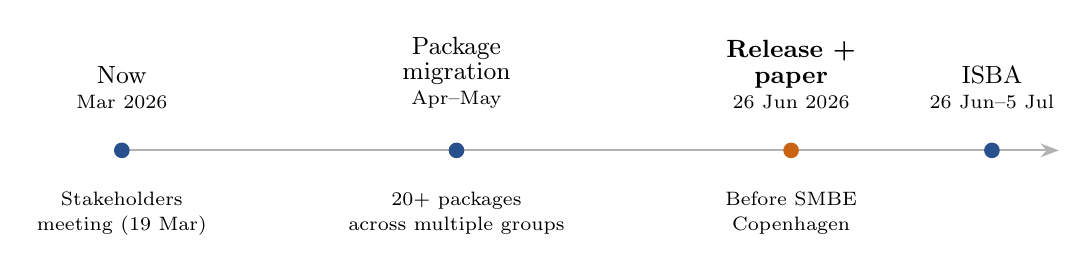
\begin{tikzpicture}[
    x=0.85cm,
    milestone/.style={circle, fill=beastblue, inner sep=2pt},
    label/.style={font=\small, align=center},
    >=Stealth
]
\draw[->, thick, gray!60] (0,0) -- (14,0);

\node[milestone] (now) at (0,0) {};
\node[label, above=0.3cm of now] {Now\\[-0.2em]\scriptsize Mar 2026};
\node[label, below=0.3cm of now] {\scriptsize Stakeholders\\[-0.2em]\scriptsize meeting (19 Mar)};

\node[milestone] (migrate) at (5,0) {};
\node[label, above=0.3cm of migrate] {Package\\[-0.2em]migration\\[-0.2em]\scriptsize Apr--May};
\node[label, below=0.3cm of migrate] {\scriptsize 20+ packages\\[-0.2em]\scriptsize across multiple groups};

\node[milestone, fill=beastorange] (release) at (10,0) {};
\node[label, above=0.3cm of release] {\textbf{Release +}\\[-0.2em]\textbf{paper}\\[-0.2em]\scriptsize 26 Jun 2026};
\node[label, below=0.3cm of release] {\scriptsize Before SMBE\\[-0.2em]\scriptsize Copenhagen};

\node[milestone] (isba) at (13,0) {};
\node[label, above=0.3cm of isba] {ISBA\\[-0.2em]\scriptsize 26 Jun--5 Jul};
\end{tikzpicture}
\end{center}
\end{frame}


% ============================================================
% 21. RESOURCES
% ============================================================

\begin{frame}{Resources}
\begin{description}
\item[Migration guide] \code{scripts/migration-guide.md}: class mapping tables, step-by-step instructions
\item[CHANGELOG] \code{CHANGELOG.md}: full list of what changed and why
\item[Package skeleton] \url{https://github.com/CompEvol/beast-package-skeleton}
\item[BEAST 3 repo] \url{https://github.com/CompEvol/beast3}
\end{description}

\vspace{1em}
\begin{block}{Migration steps}
\begin{enumerate}
\item Create \code{pom.xml} (see skeleton), target Java 25
\item Fix compile errors (\code{StateNode}/\code{Function}, \code{scale()}, \code{Evaluator})
\item Add \code{module-info.java} with \code{provides} declarations
\item Migrate to spec types incrementally
\end{enumerate}
\end{block}
\end{frame}

\end{document}
